\section{Empirical Probabilities and Realistic Seat Layouts}\label{appen_3}
\subsection{Empirical Probabilities}
We select Movie A (representing the suspense genre) and Movie B (representing the family fun genre) as target movies to analyze group information and their corresponding probability distributions, denoted as $D3$ and $D4$, respectively.

% The seat plans for the tickets were obtained from a Hong Kong cinema website. We focused on scattered seat plans and excluded cases where the number of consecutive seats exceeded four. By counting the occurrences of different group types, we obtained these distributions. 

% $\hat{p}_i \pm z_{\alpha / 2} \sqrt{\frac{\hat{p}_i\left(1-\hat{p}_i\right)}{N}} = $
% 0.122 $\pm$ 0.011
% 0.501 $\pm$ 0.016
% 0.132 $\pm$ 0.011
% 0.246 $\pm$ 0.014

% Similarly, 

% 0.336 $\pm$ 0.025
% 0.516 $\pm$ 0.027
% 0.067 $\pm$ 0.013
% 0.081 $\pm$ 0.015


We make the screenshots about the ticket seat plans from a Hong Kong cinema website at different time intervals. When tickets were sold in advance of the movie screening, the seats were typically scattered. Therefore, we treated consecutive seats as belonging to the same group, while excluding cases where the number of consecutive seats exceeds four. 

We counted the frequency of different group types in the seat plans to derive their probability distributions. For Movie A, the frequencies for the four group types are 112, 460, 121, and 226, with a total of 919 observations. For Movie B, the frequencies are 116, 178, 23, and 28, with a total of 345 observations. We keep two decimal places, then obtain the probability:

$p_1^{A} =  0.12$, $p_2^{A} =  0.50$, $p_3^{A} = 0.13$, $p_4^{A} = 0.25$ and $p_1^{B} =  0.34$, $p_2^{B} =  0.52$, $p_3^{B} = 0.07$, $p_4^{B} = 0.08$.

% ${p}_i \pm z_{\alpha / 2} \sqrt{\frac{{p}_i\left(1-{p}_i\right)}{N}}, z_{\alpha / 2} = 1.96$

Using the normal distribution approximation method (with a 95\% confidence interval), the confidence intervals for the probabilities of each group type for Movie A is presented as follows:
$CI_1^{A} =  0.122 \pm 0.011$, $CI_2^{A} =  0.501 \pm 0.016$, $CI_3^{A} = 0.132 \pm 0.011$, $CI_4^{A} = 0.246 \pm 0.014$

Similarly, the confidence intervals for the probabilities of each group type for Movie B are:

$CI_1^{B} =  0.336 \pm 0.025$, $CI_2^{B} =  0.516 \pm 0.027$, $CI_3^{B} = 0.067 \pm 0.013$, $CI_4^{B} = 0.081 \pm 0.015$


% HKFAC, KTTTS, SWHCC, SWCC, NCWCC

% https://www.lcsd.gov.hk/en/ticket/seat.html

\subsection{Realistic Seat Layouts}

\begin{figure}[ht]
  \caption{Layout A}
    \centering
      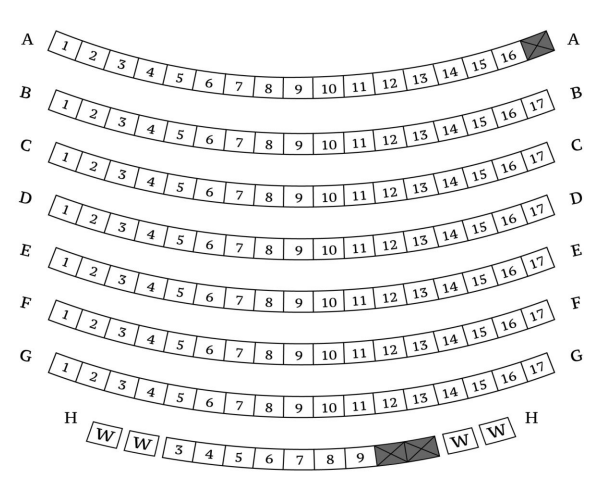
\includegraphics[width=0.6\textwidth]{./Figures/Layouts/Layout_A.png}
\end{figure}
  
\begin{figure}[ht]
  \caption{Layout B}
    \centering
      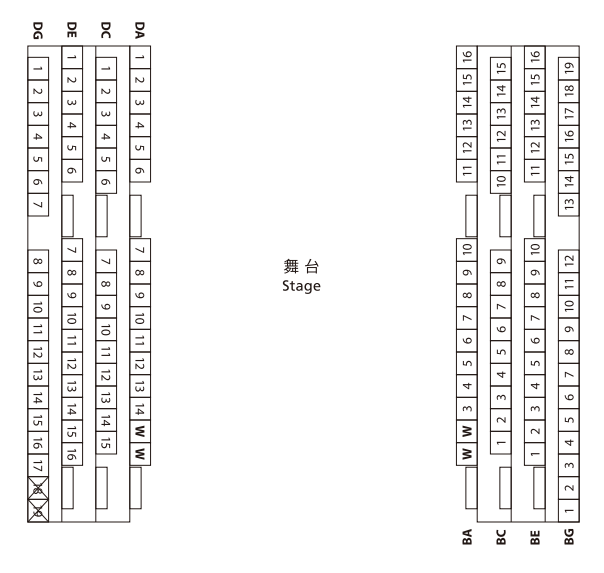
\includegraphics[width=0.6\textwidth]{./Figures/Layouts/Layout_B.png}
\end{figure}

\begin{figure}[ht]
  \caption{Layout C}
    \centering
      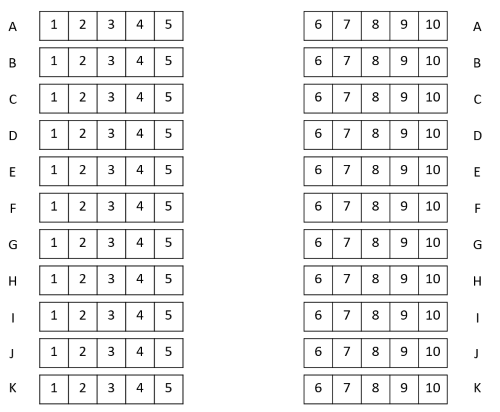
\includegraphics[width=0.6\textwidth]{./Figures/Layouts/Layout_C1.png}
\end{figure}

\begin{figure}[ht]
  \caption{Layout D}
    \centering
      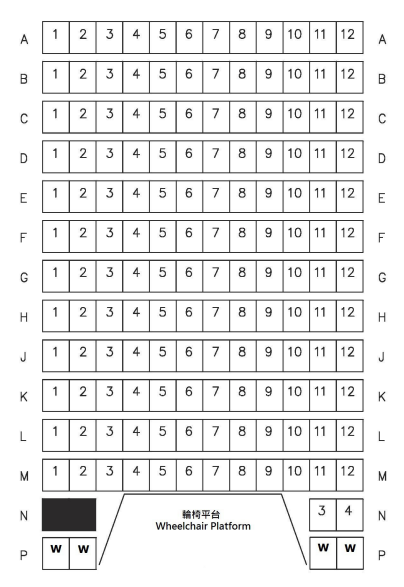
\includegraphics[width=0.6\textwidth]{./Figures/Layouts/Layout_D.png}
\end{figure}

\begin{figure}[ht]
  \caption{Layout E}
    \centering
      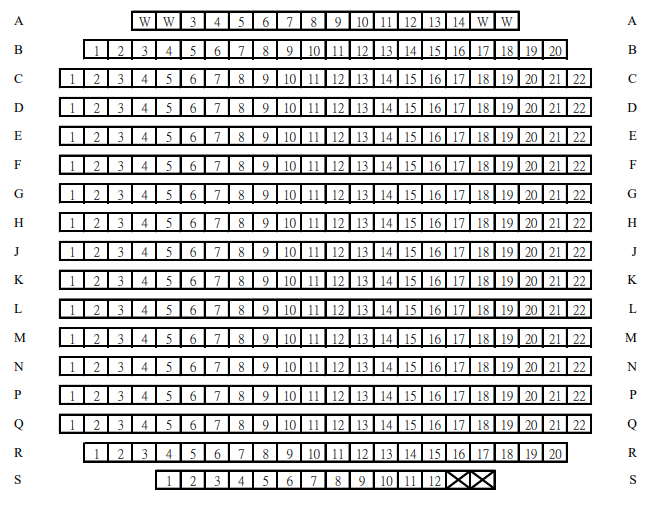
\includegraphics[width=0.6\textwidth]{./Figures/Layouts/Layout_E.png}
\end{figure}
